\pagebreak
\subsection{Implementing Mach Number Jumps}
% [25\%] Implement the mesh adaptation algorithm based on the Mach number jumps. Run your algorithm for $\alpha = 1\degree$ with at least 5 adaptive iterations, and perform the following post-processing: Plot the sequence of your adapted meshes. Plot the Mach number and total pressure fields on your finest mesh. Plot the ATPR output versus number of cells in the mesh -- one data point per adaptive iteration.

Discuss the results, including areas targeted for adaption and the convergence of the output.

\subsubsection{Adapted Meshes}

\begin{figure}[h]
    \centering
    \begin{subfigure}[h]{0.32\linewidth}
        \centering
        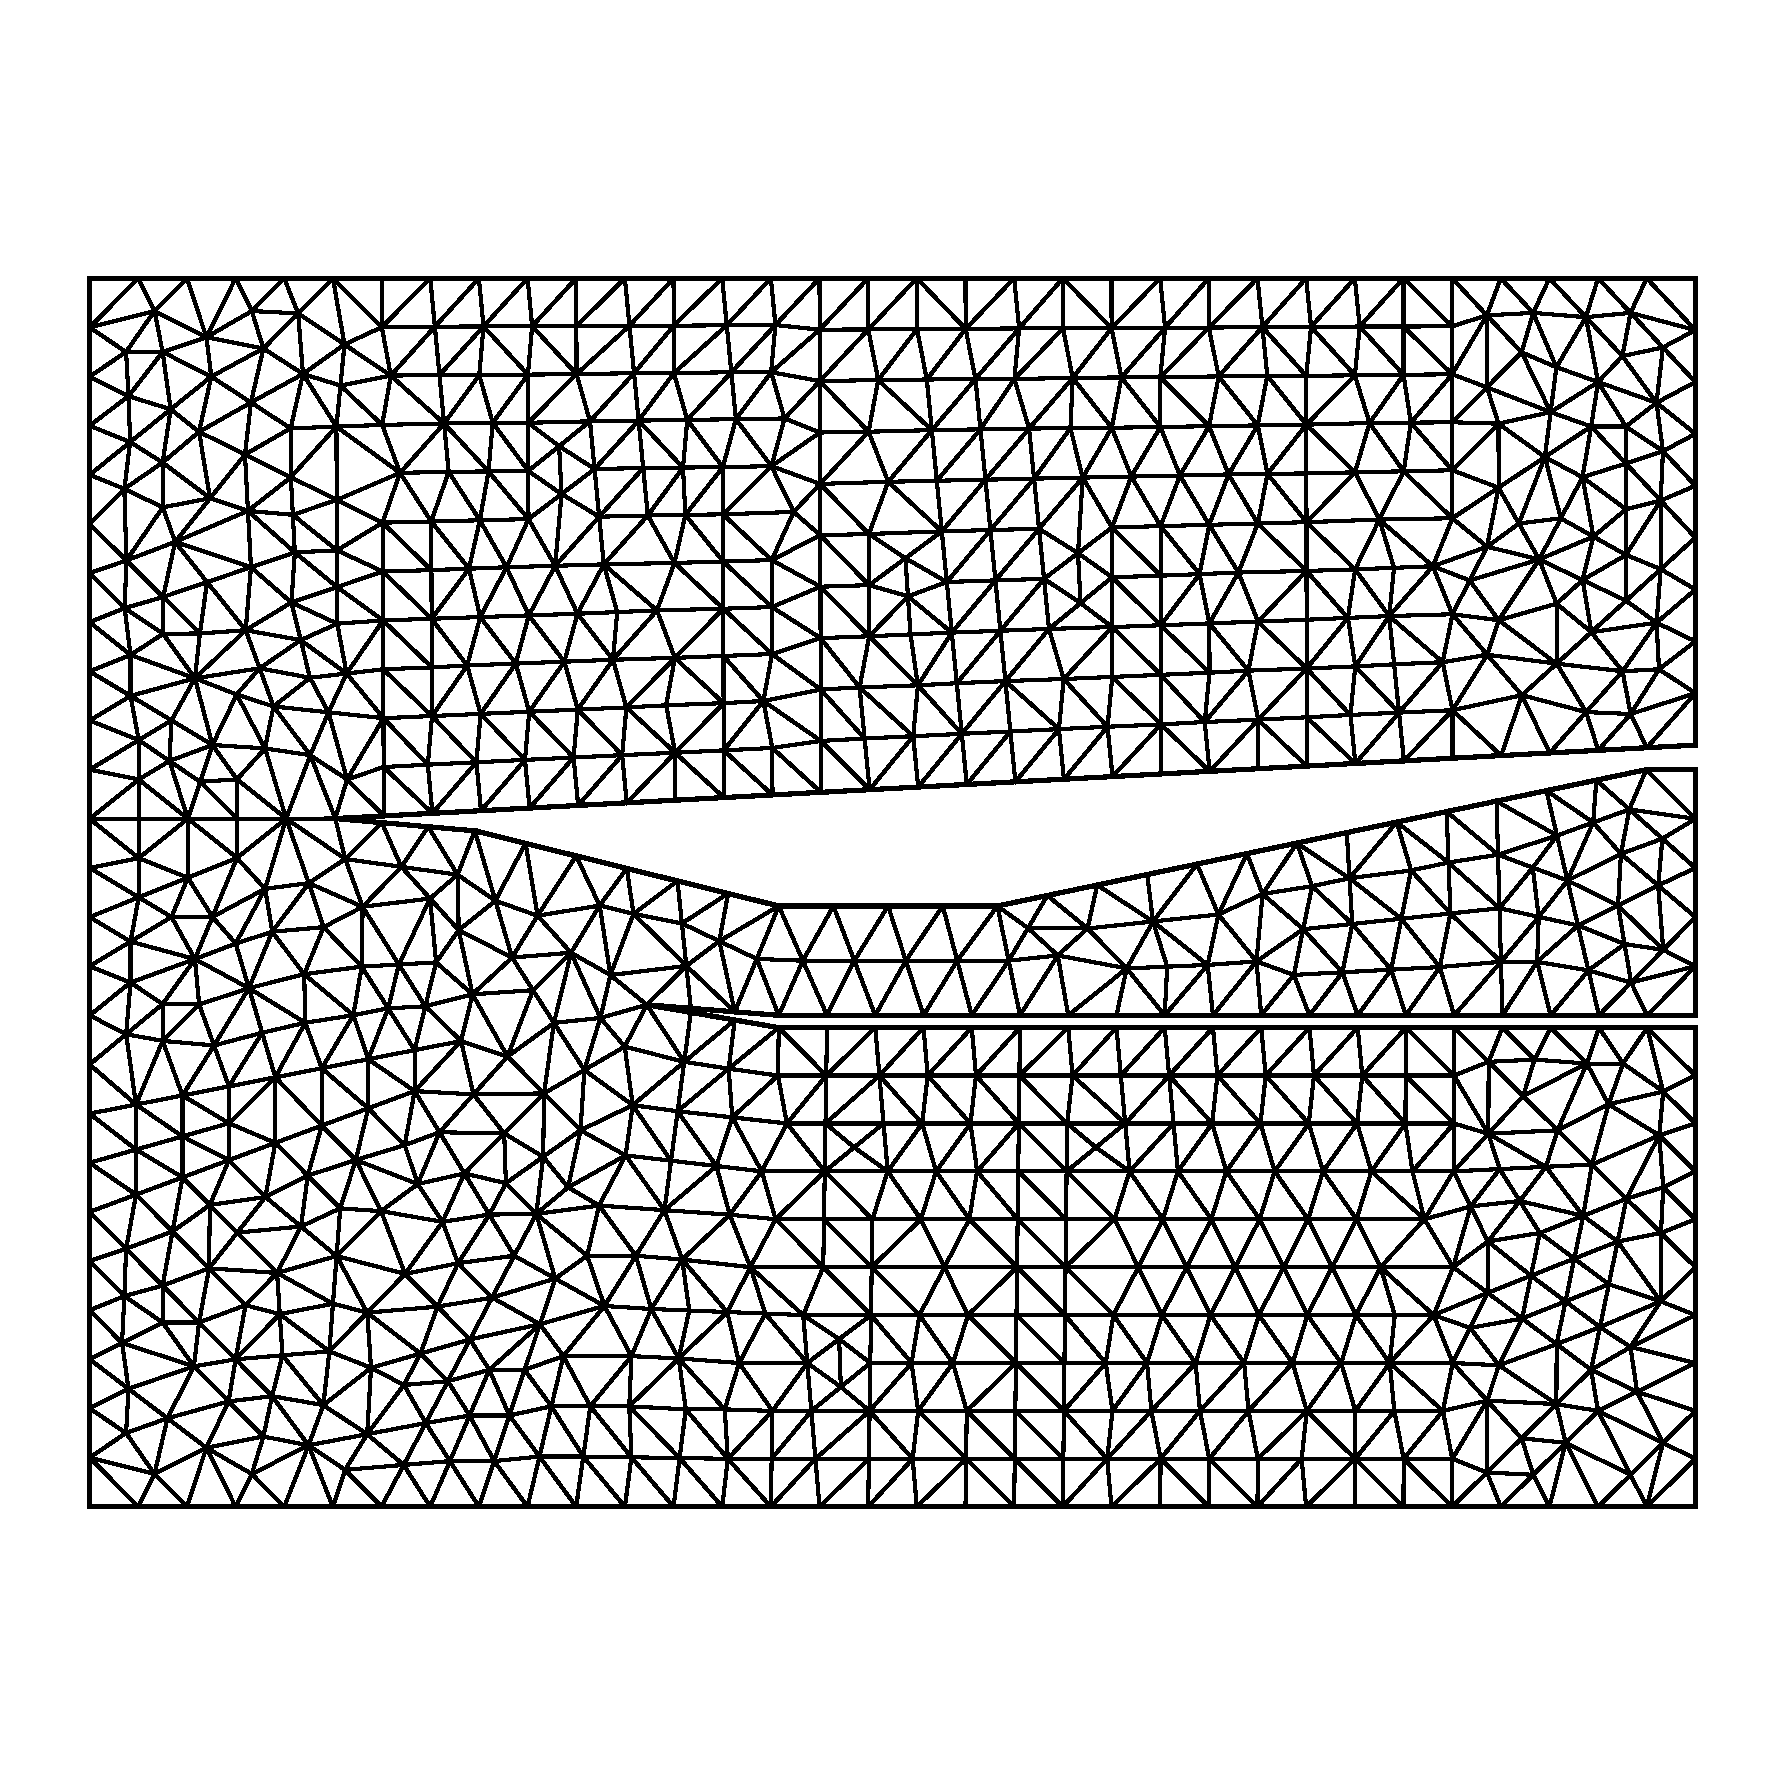
\includegraphics[width=\linewidth]{rep/q4/mesh0.pdf}
        \caption{Baseline mesh.}
    \end{subfigure}
    \begin{subfigure}[h]{0.32\linewidth}
        \centering
        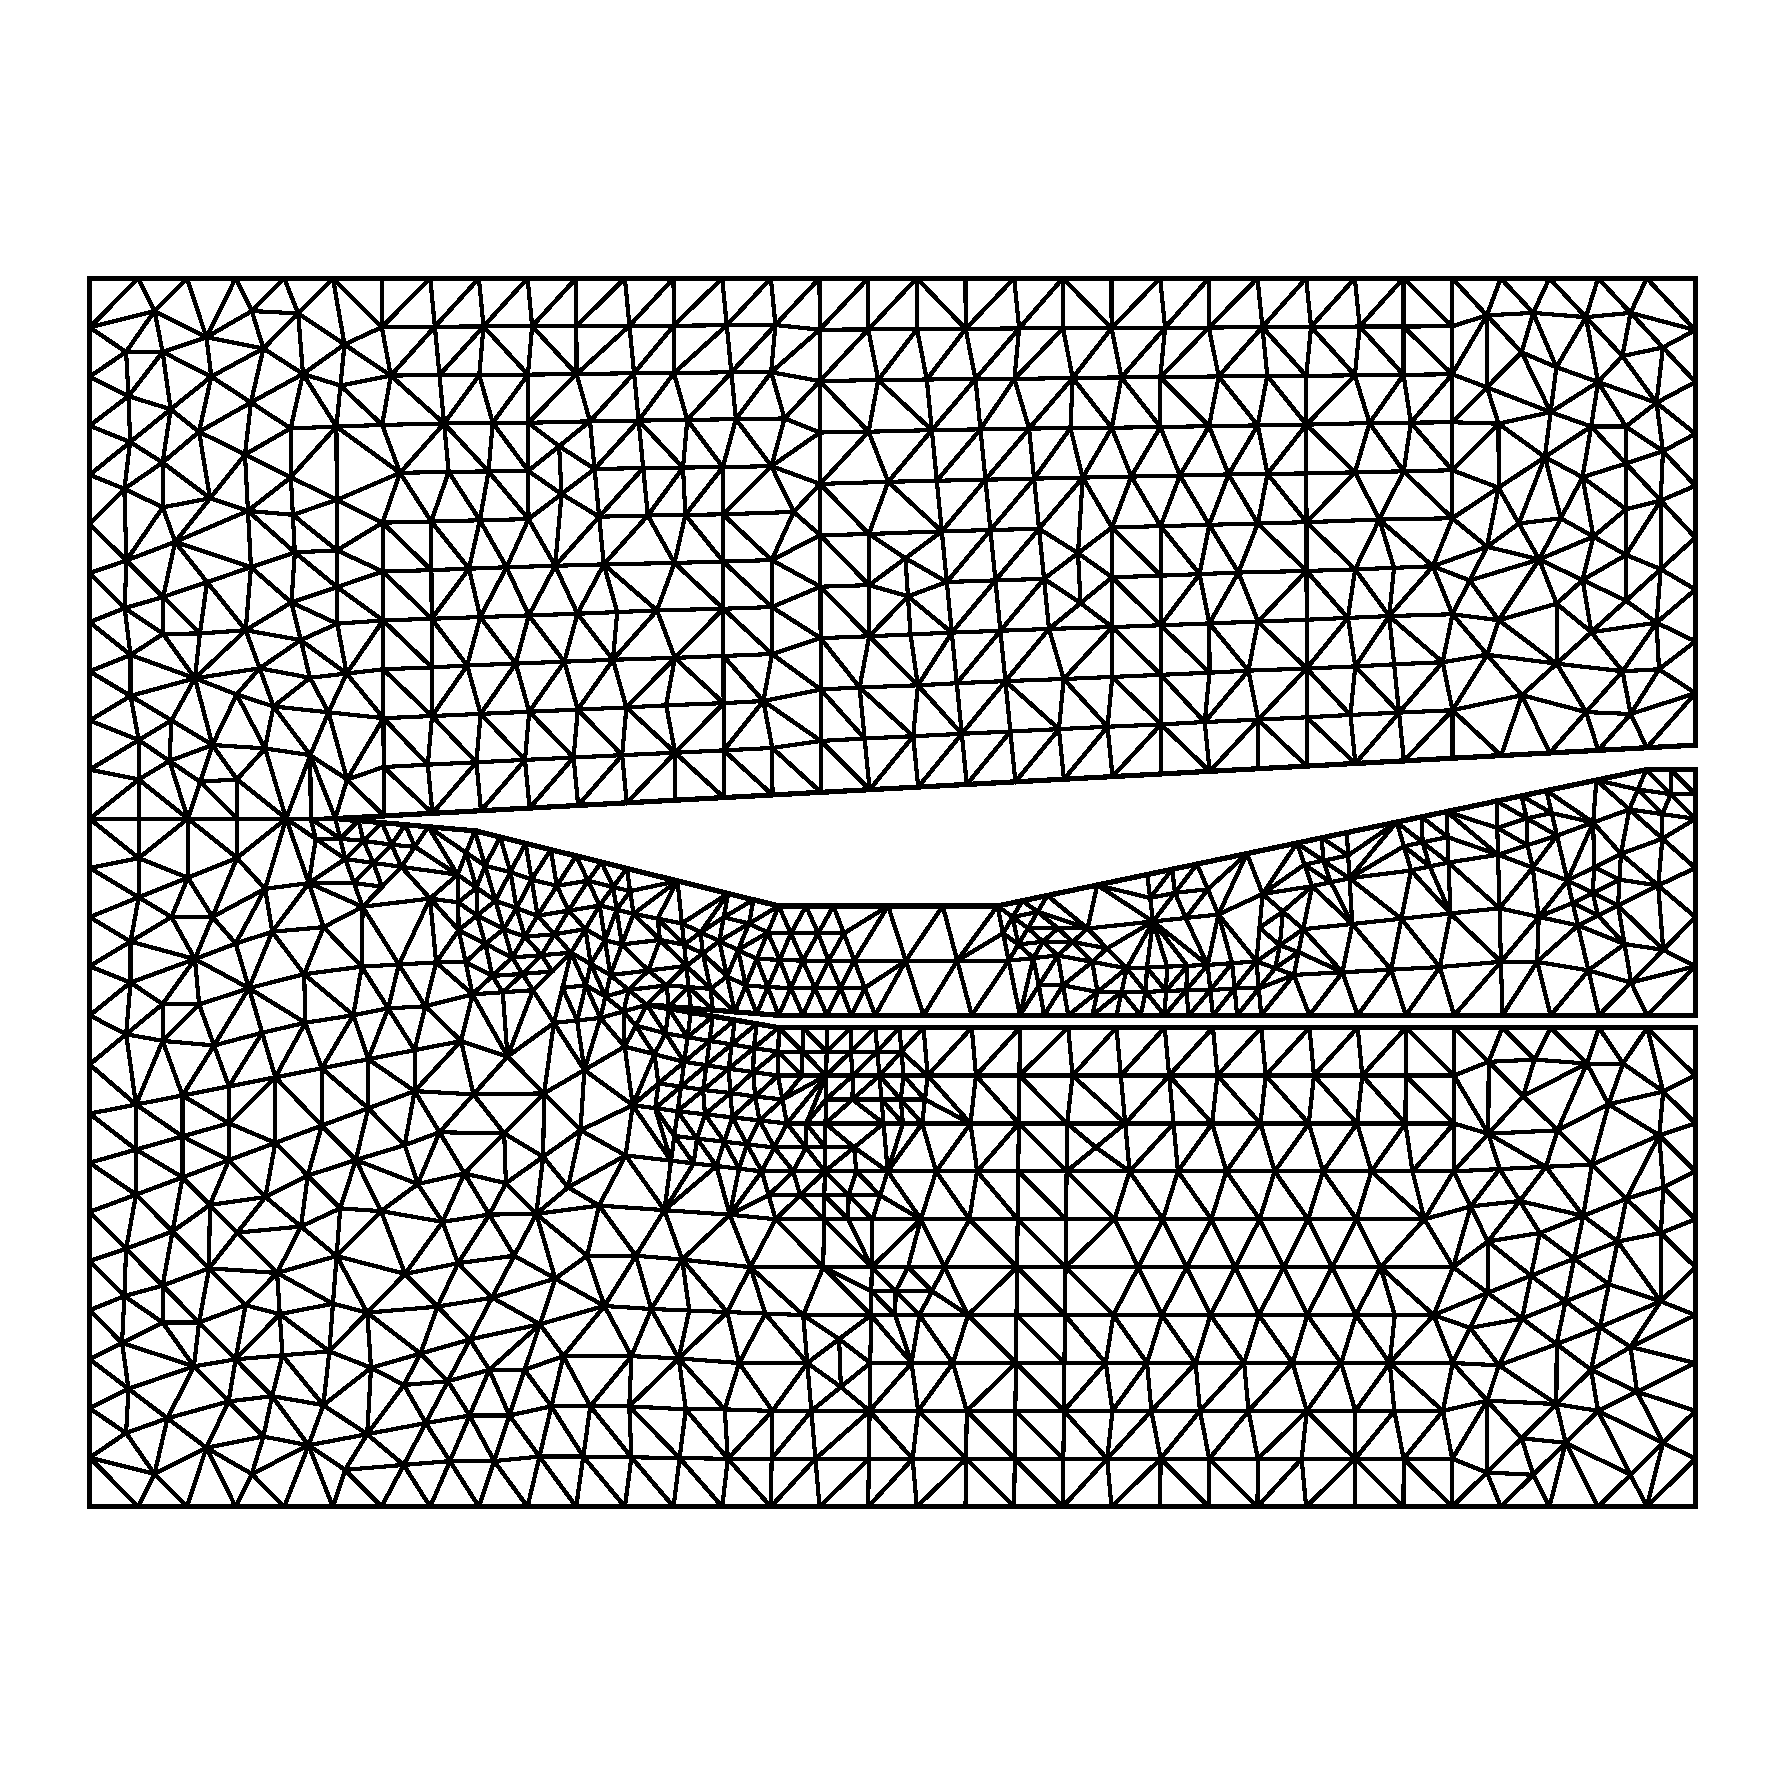
\includegraphics[width=\linewidth]{rep/q4/mesh1.pdf}
        \caption{Adapted mesh, iteration 1.}
    \end{subfigure}
    \begin{subfigure}[h]{0.32\linewidth}
        \centering
        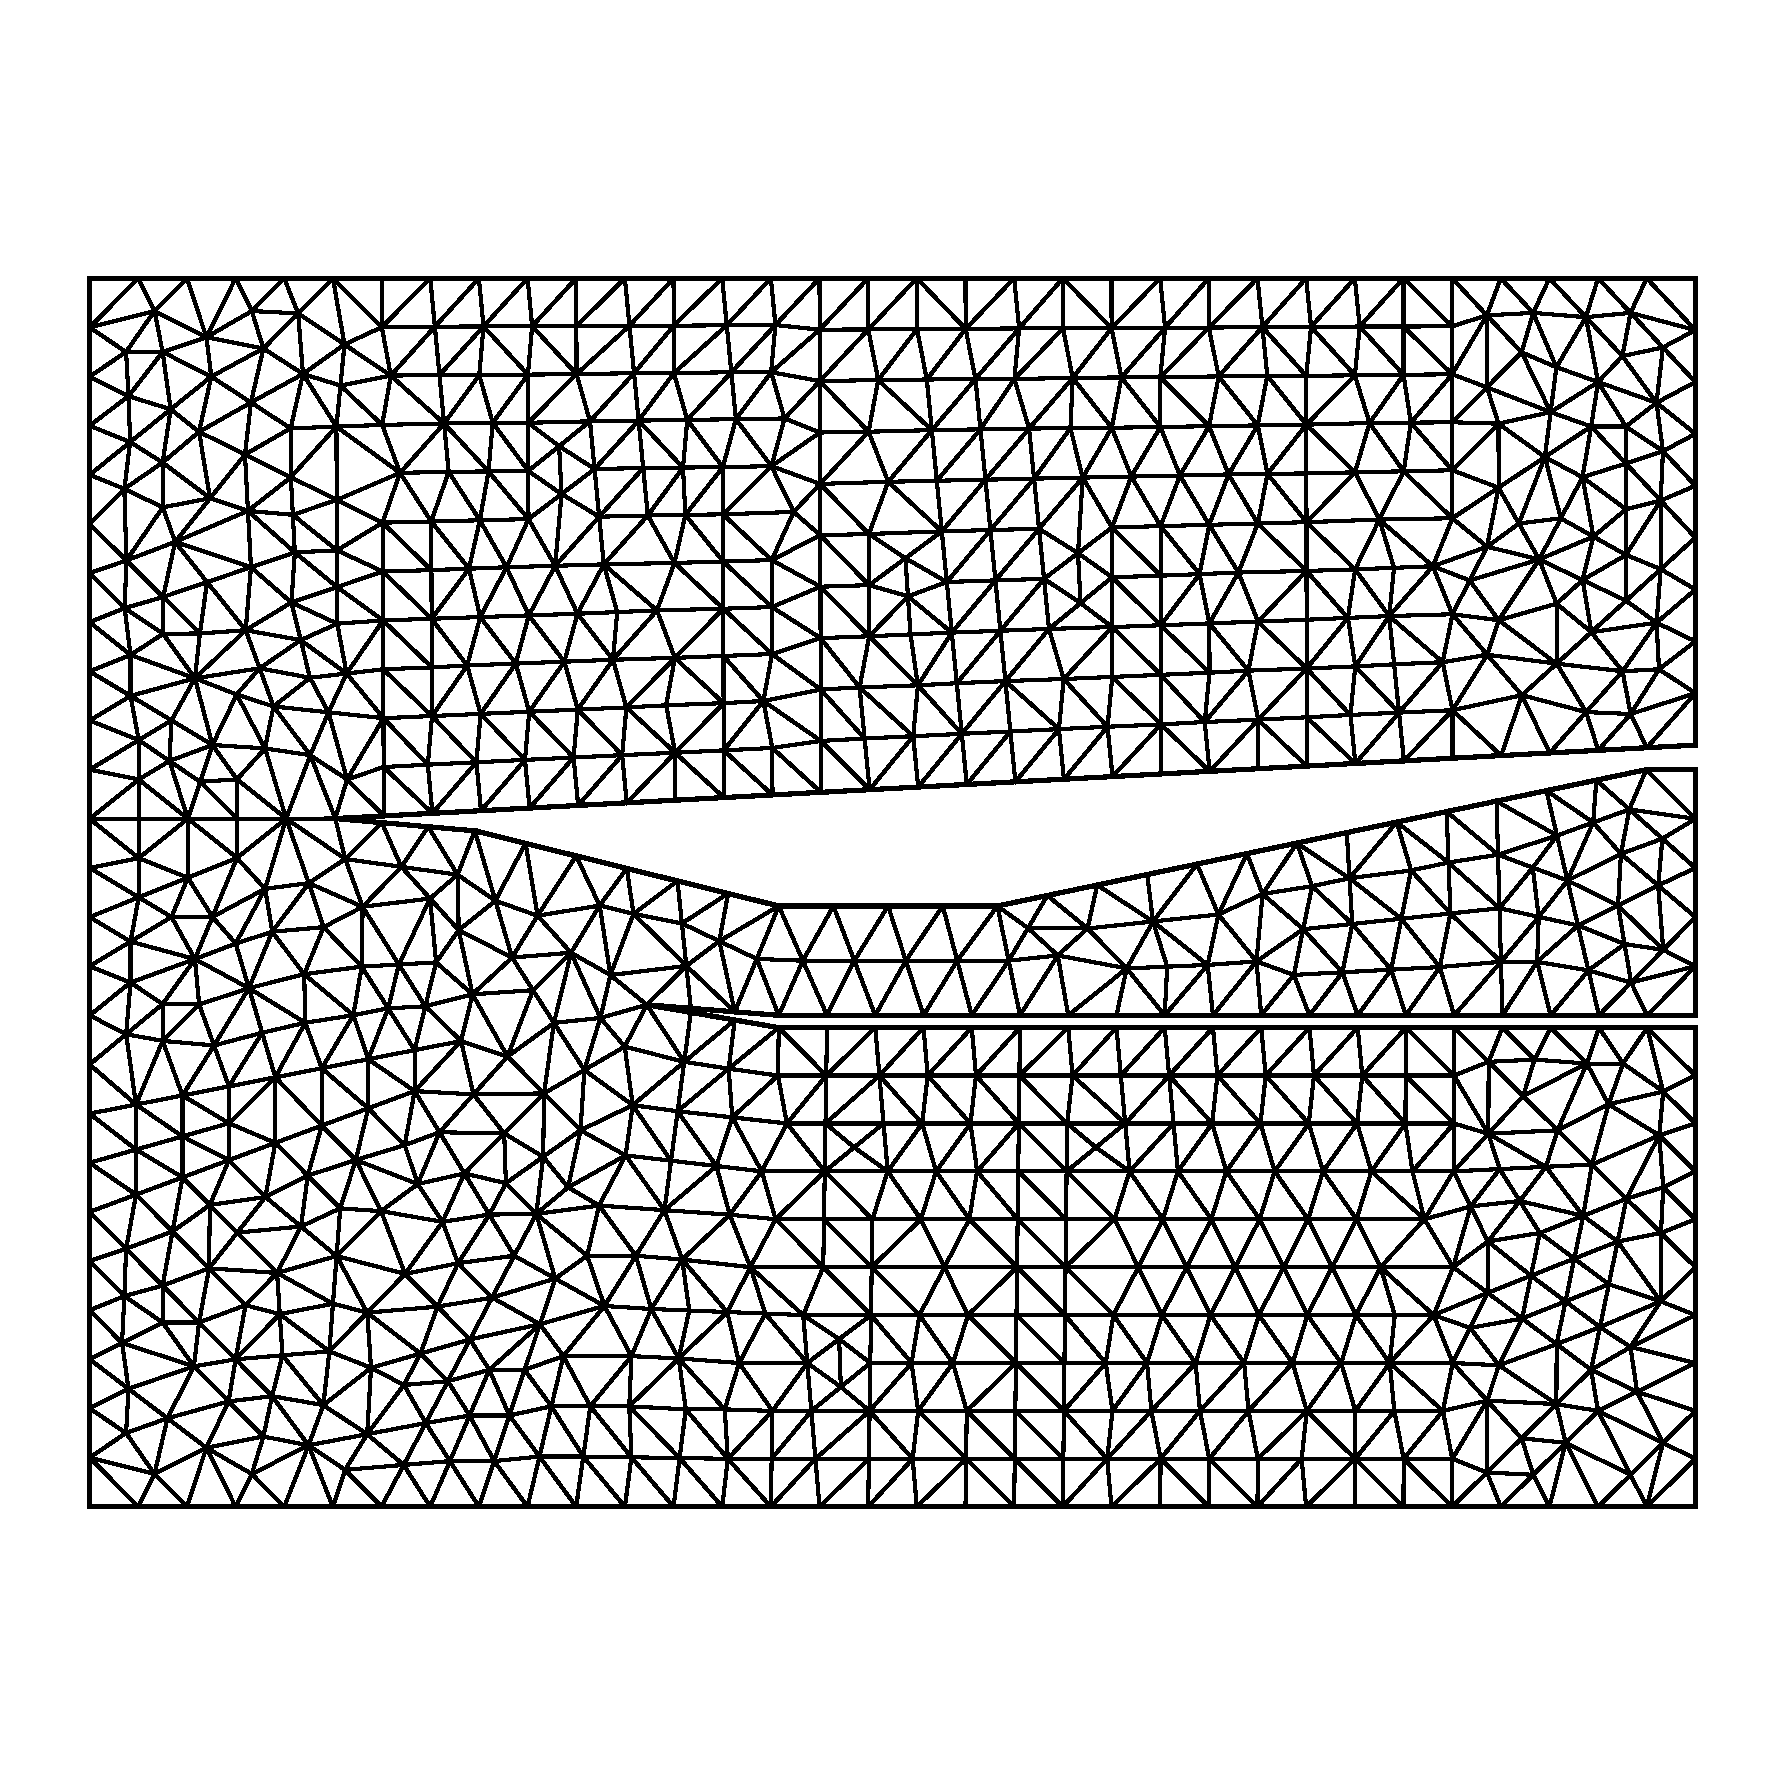
\includegraphics[width=\linewidth]{rep/q4/mesh2.pdf}
        \caption{Adapted mesh, iteration 2.}
    \end{subfigure}

    \begin{subfigure}[h]{0.32\linewidth}
        \centering
        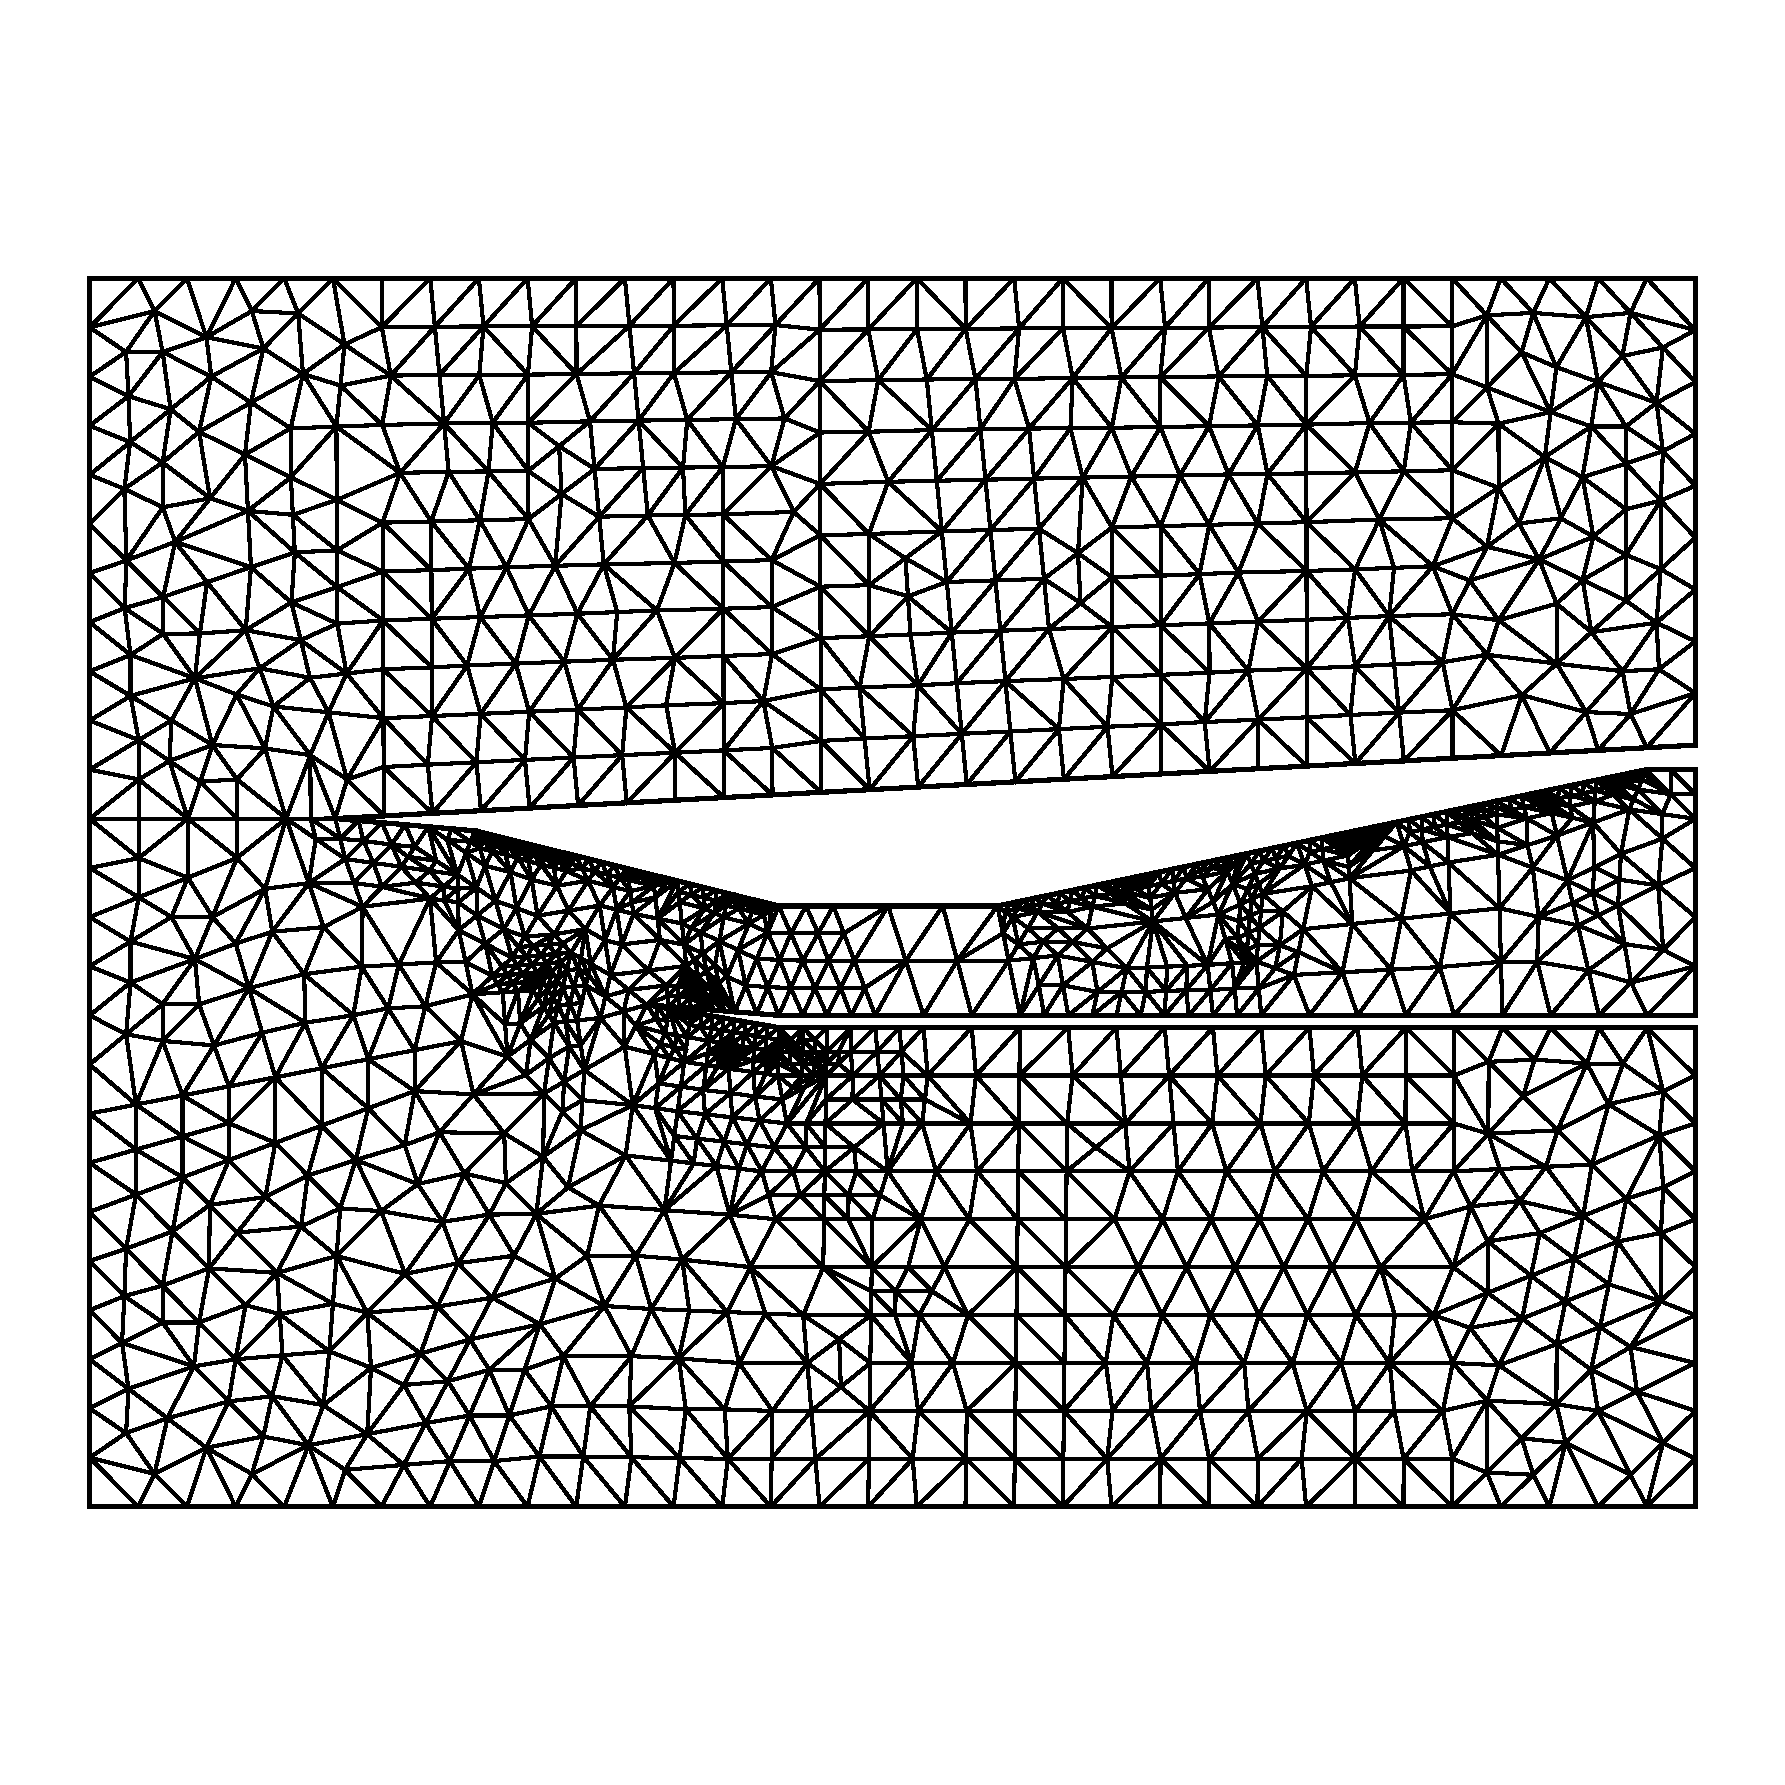
\includegraphics[width=\linewidth]{rep/q4/mesh3.pdf}
        \caption{Adapted mesh, iteration 3.}
    \end{subfigure}
    \begin{subfigure}[h]{0.32\linewidth}
        \centering
        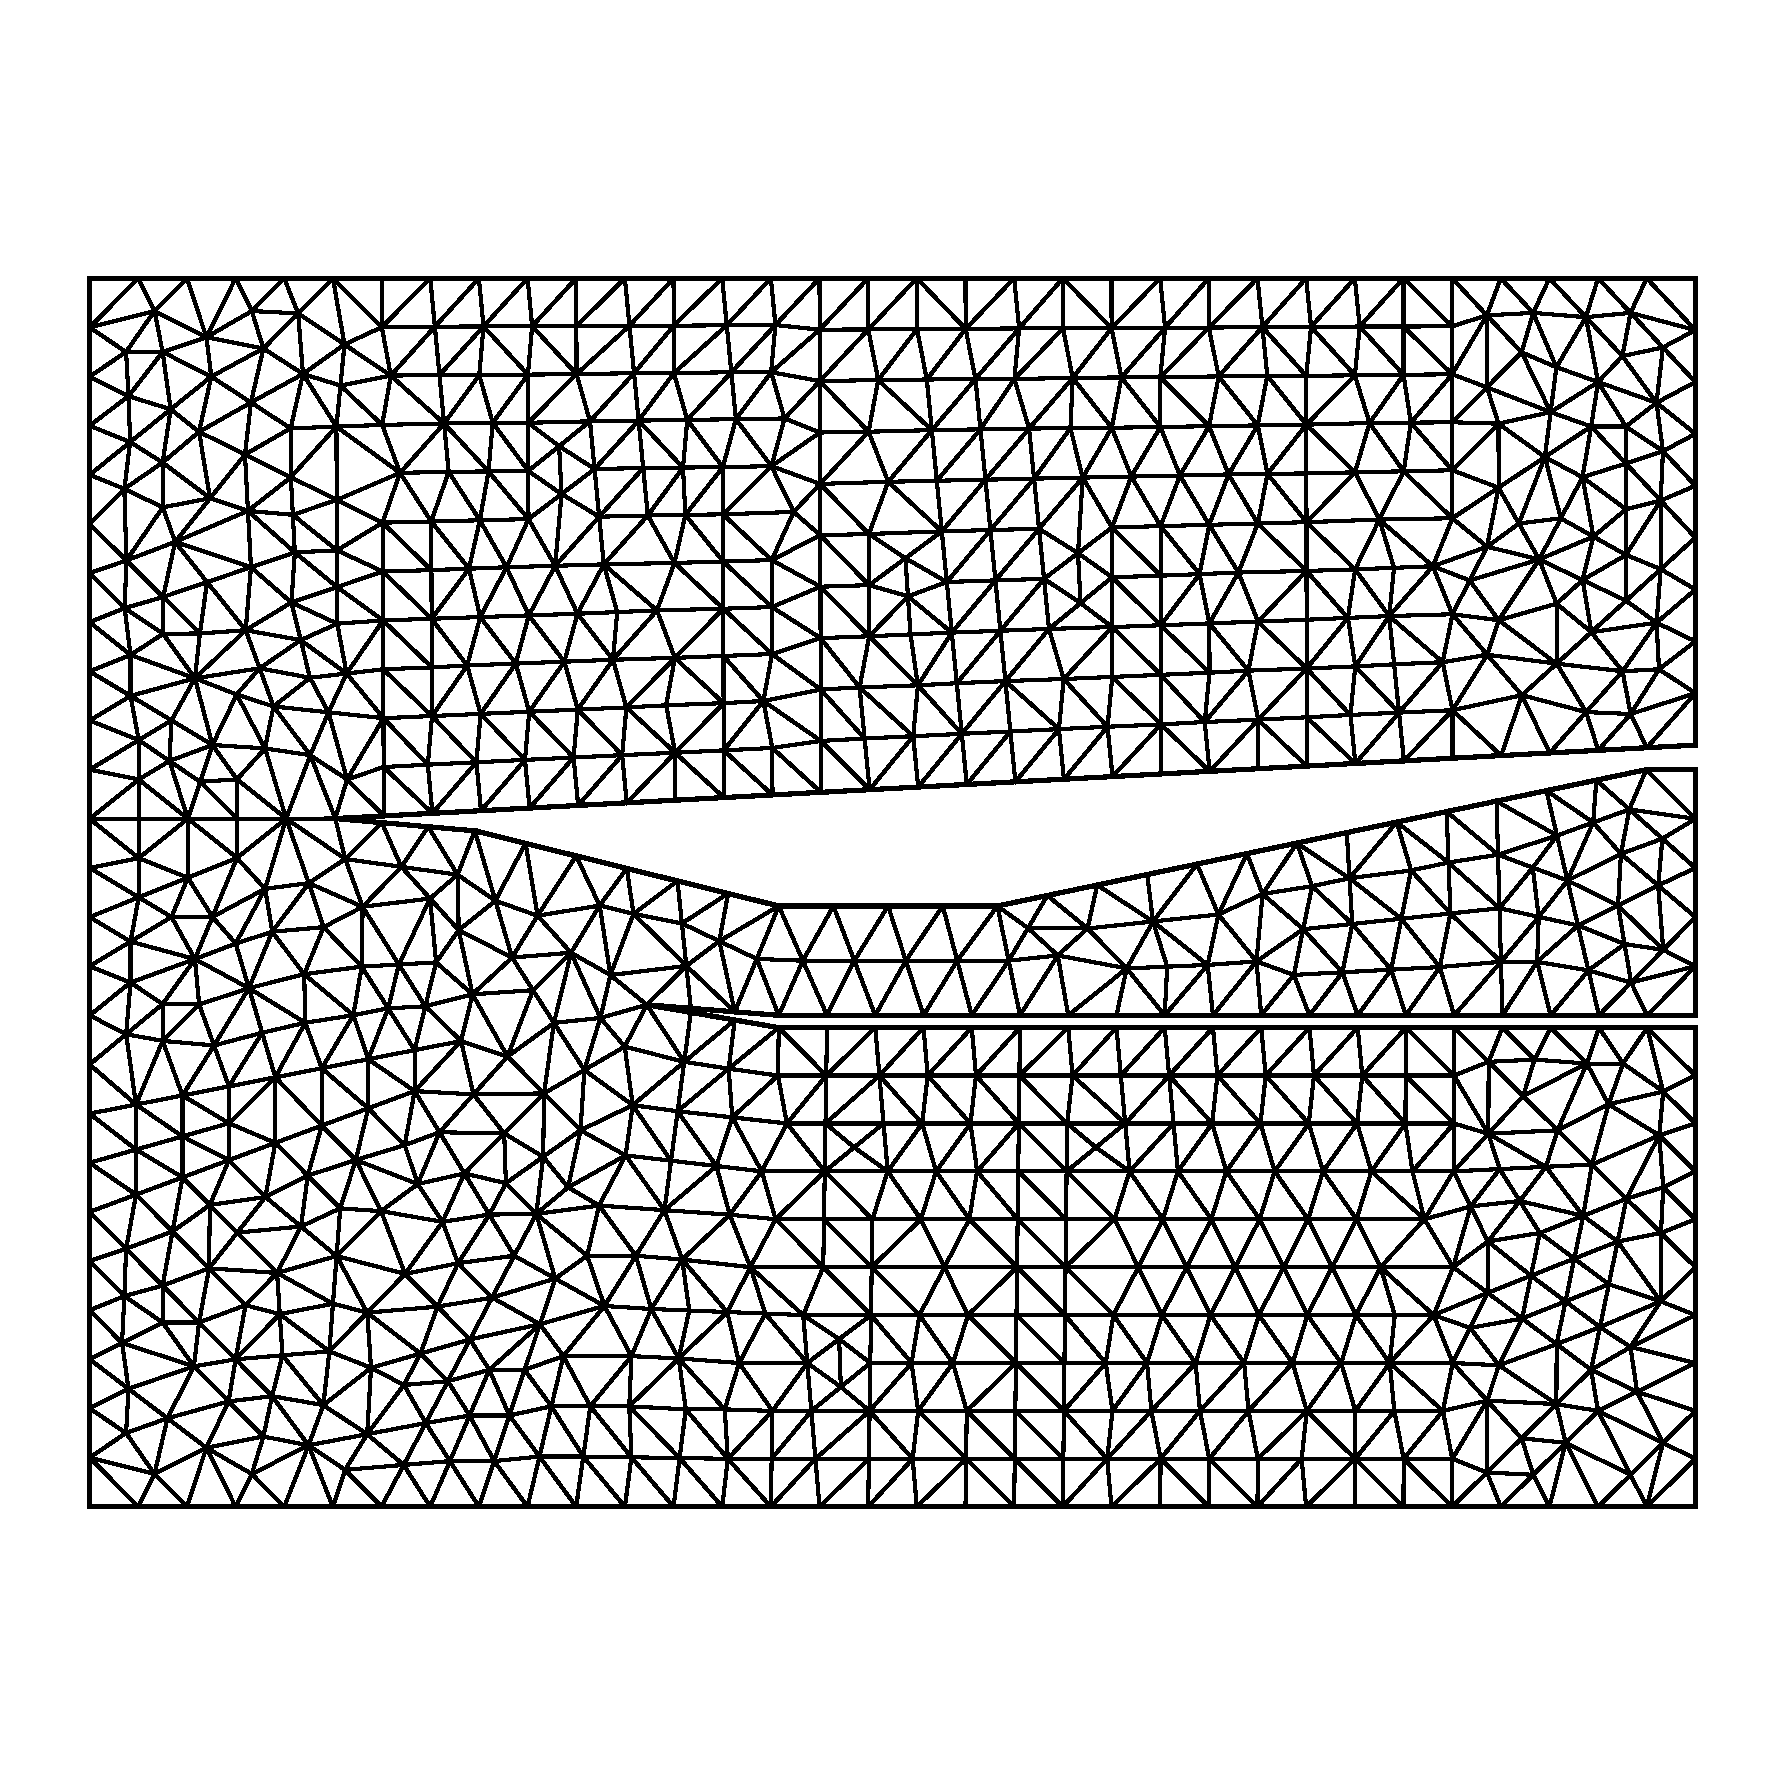
\includegraphics[width=\linewidth]{rep/q4/mesh4.pdf}
        \caption{Adapted mesh, iteration 4.}
    \end{subfigure}
    \begin{subfigure}[h]{0.32\linewidth}
        \centering
        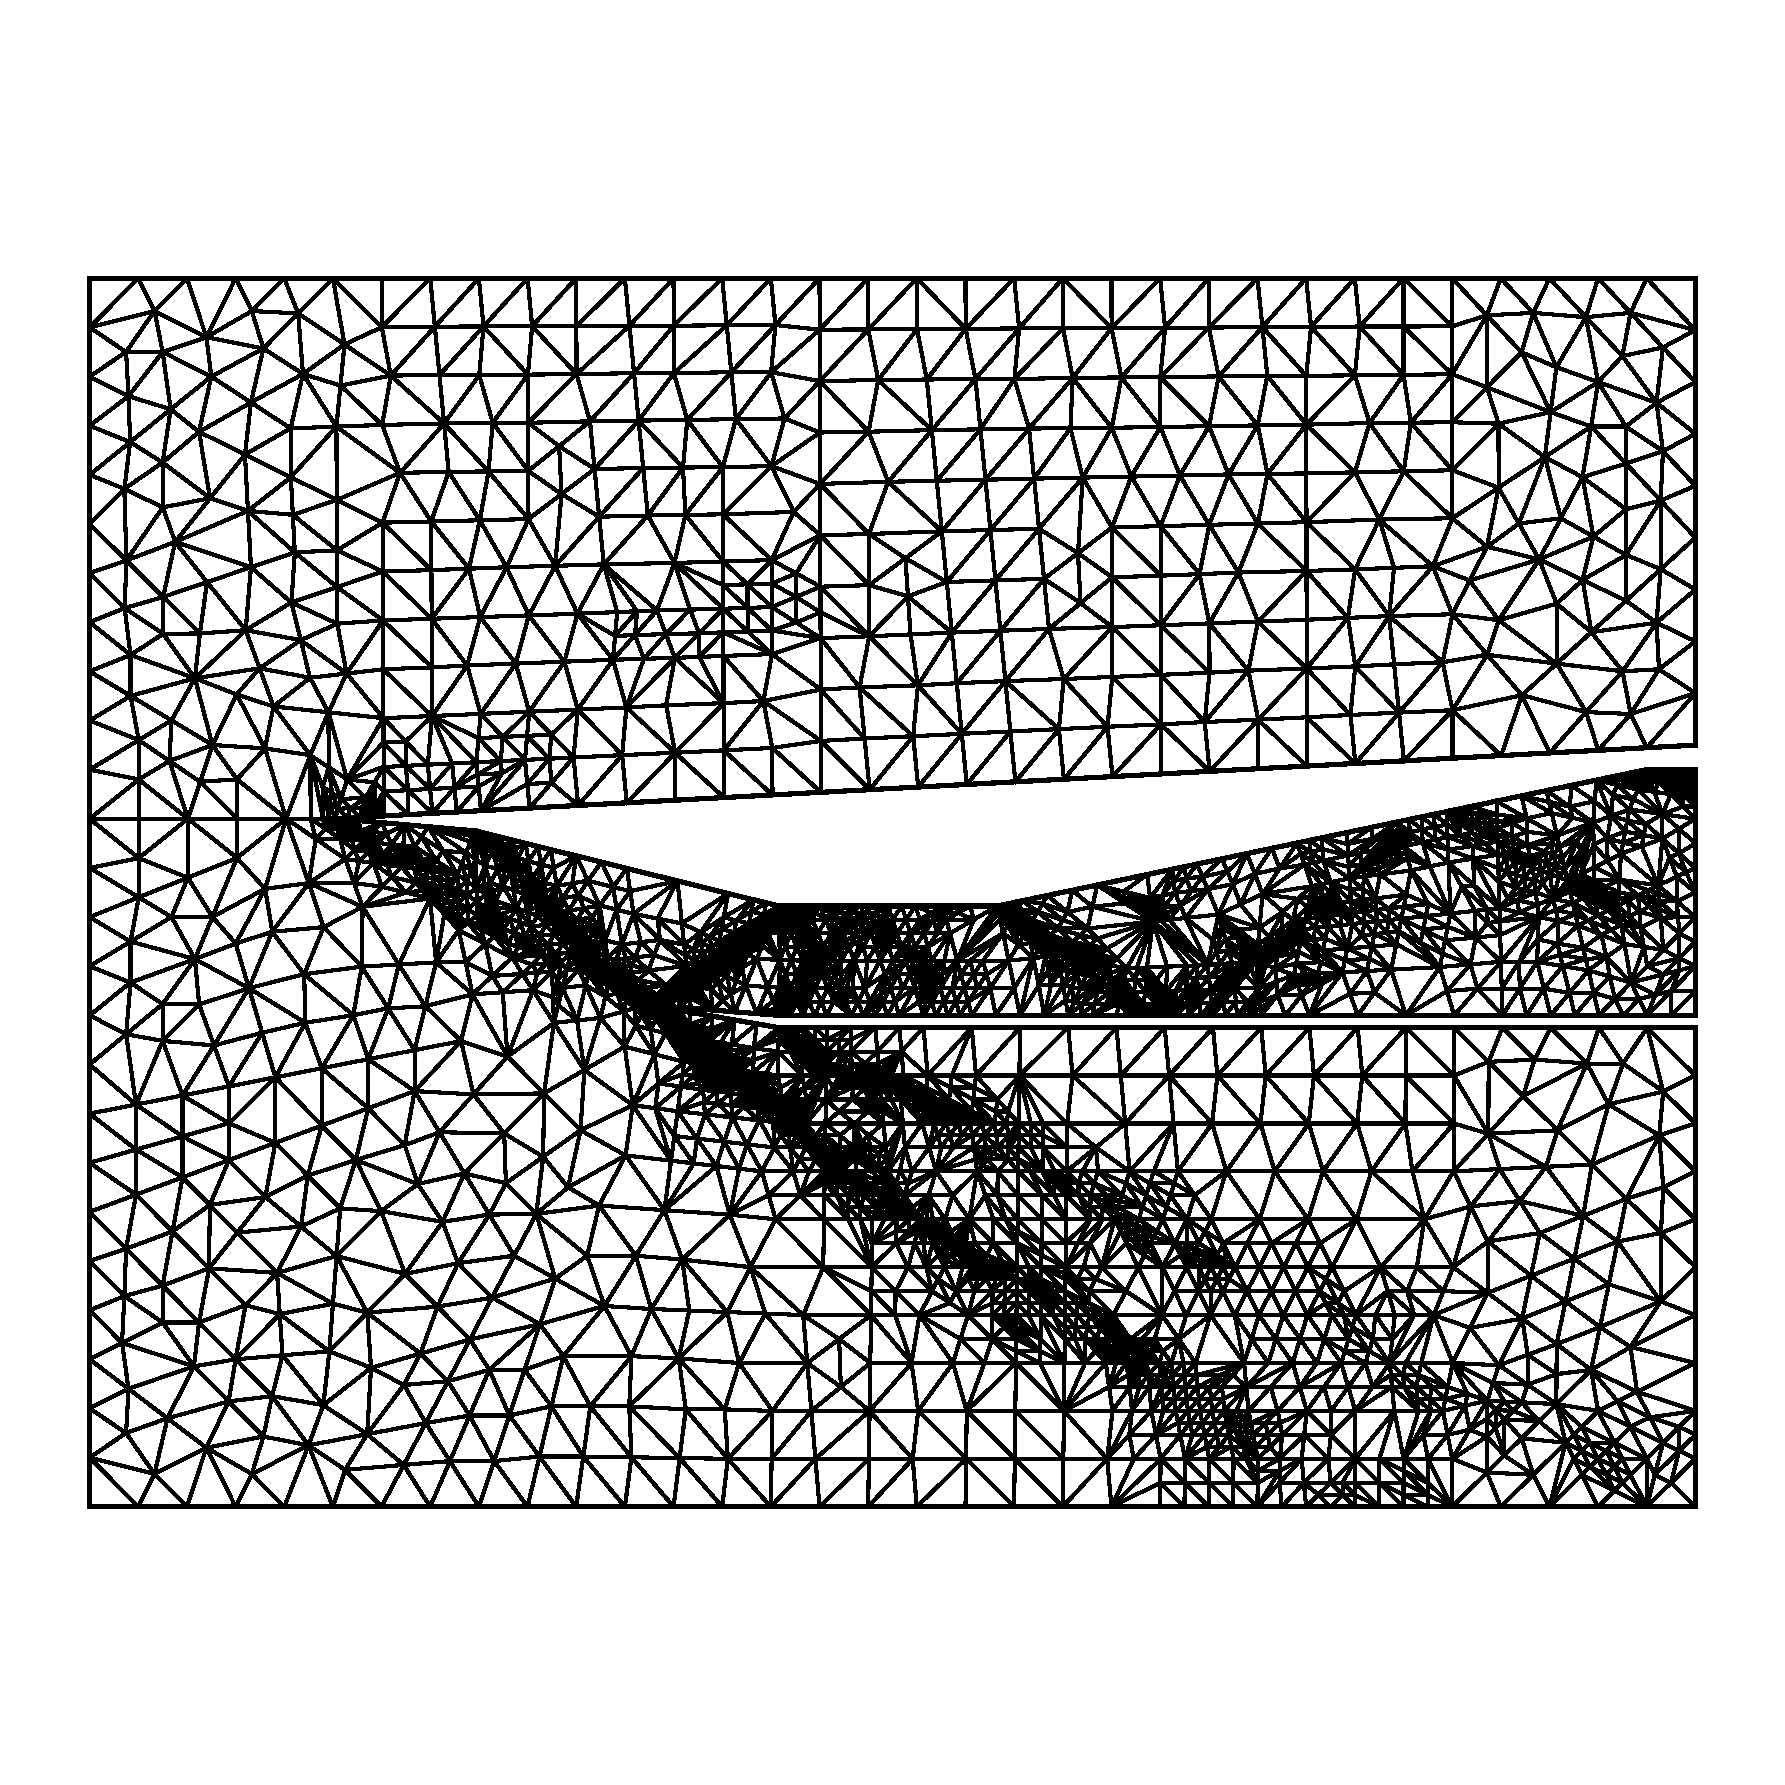
\includegraphics[width=\linewidth]{rep/q4/mesh5.pdf}
        \caption{Adapted mesh, iteration 5.}
    \end{subfigure}
    \caption[Adapted Meshes Versus Baseline Mesh]{Adapted meshes versus baseline mesh.}
    \label{fig:adapted_meshes}
\end{figure}

\textcolor{red}{\large PLACE HOLDER}

\pagebreak
\subsubsection{Adapted Mesh Field Plots}
\begin{figure}[h]
    \centering
    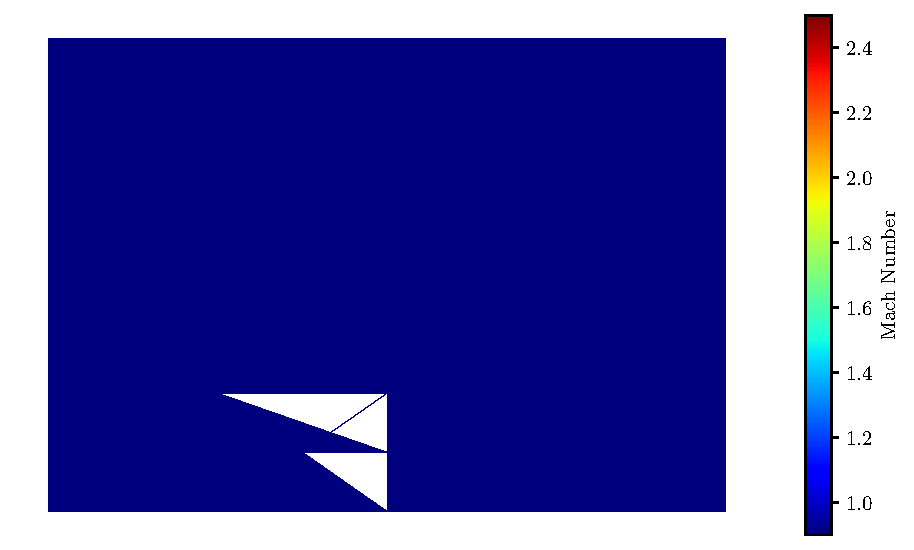
\includegraphics[width = 0.9\linewidth]{rep/q4/Machfield.pdf}
    \caption[Field Plot of Mach Number for Adapted Mesh]{Field plot of Mach number with $\alpha = 1\degree$ for the finest mesh.}
    \label{fig:adapted_mach}
\end{figure}

\textcolor{red}{\large PLACE HOLDER}

\pagebreak
\begin{figure}[h]
    \centering
    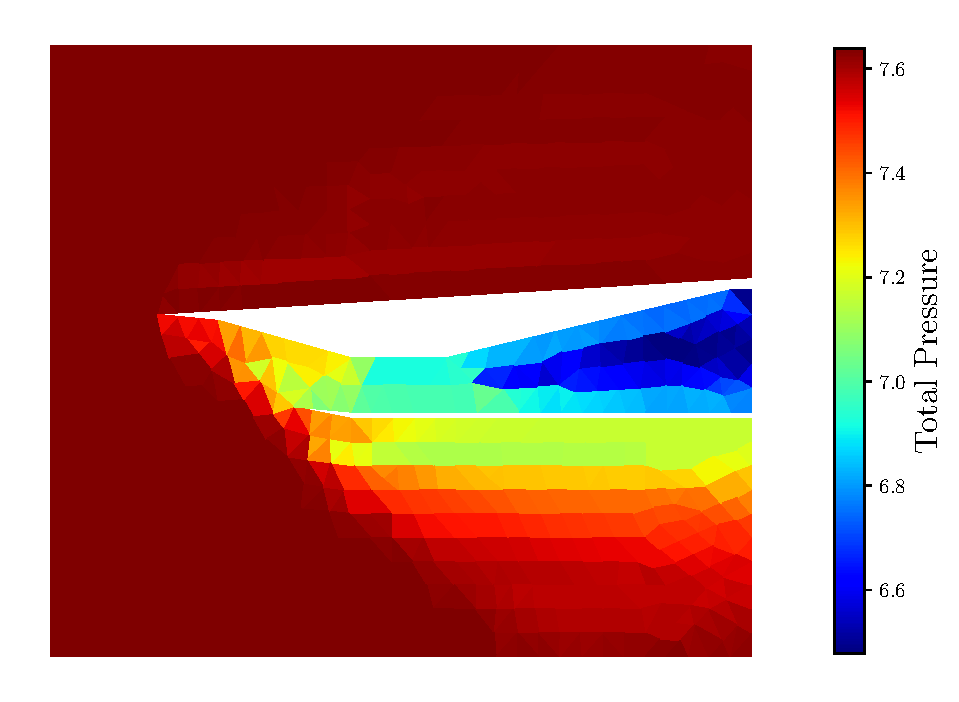
\includegraphics[width = 0.9\linewidth]{rep/q4/Pfield.pdf}
    \caption[Field Plot of Total Pressure for Adapted Mesh]{Field plot of total pressure with $\alpha = 1\degree$ for the finest mesh.}
    \label{fig:adapted_pt}
\end{figure}

\textcolor{red}{\large PLACE HOLDER}

\pagebreak
\subsubsection{Adapted Mesh ATPR Convergence}
\begin{figure}[h]
    \centering
    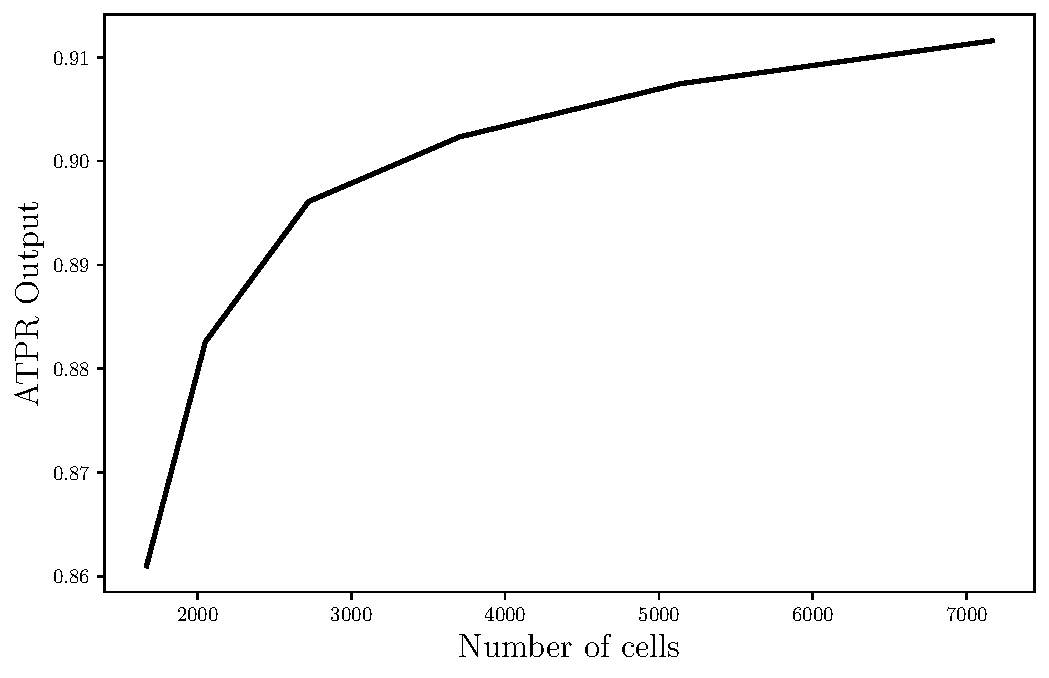
\includegraphics[width = 0.9\linewidth]{rep/q4/ATPR.pdf}
    \caption[ATPR Convergence with Cell Number]{ATPR output versus number of cells in mesh.}
    \label{fig:adapted_ATPR}
\end{figure}

\textcolor{red}{\large PLACE HOLDER}